\documentclass[11pt, draft]{beamer}

\usepackage[T1]{fontenc}
% \usepackage{lmodern}

% \usepackage{mathptmx}
% \usepackage{helvet}
% \renewcommand{\rmdefault}{ptm}



\usepackage[final]{listings}
\usepackage{verbatim}
\usepackage{xcolor}
\usepackage{multirow}
\usepackage{multicol}
\usepackage{pgfplots}
\usepackage[normalem]{ulem}
\usepackage[english]{babel}
\usepackage{times}
\usepackage{tikz}
% \usepackage{tabularx}

% --- Setttings
\graphicspath{{figs/}}

% --- Listings
\lstset{escapeinside={(*@}{@*)}}
\lstdefinestyle{lara}{language=C++,
  frame=single, frameround=tttt,
  rulecolor=\color{lightgray},
  morekeywords={aspectdef, var, apply, select, condition, begin, end, input, entry, exit}}
\lstdefinestyle{MaxC}{language=C++,
  morekeywords={s_int32, int32, float8_24, sin_float8_24,
    sout_float8_24, float8_24, s_int, s_float8_24, s_bool, count, countChain,
    CURRENT_CYCLE, MAX_CYCLE, pragma},
  deletekeywords={static}}
\lstdefinestyle{MaxJ}{
  morekeywords={HWVar, io, hwFloat, stream}
}

\lstset{
  basicstyle=\footnotesize,
  keywordstyle=\color{black}\bfseries,
  captionpos=b,
  breaklines=true,
  showspaces=false,
  escapeinside={(*@}{@*)}
}

% --- PGF Plots ---
\pgfplotsset{
  width=0.9\textwidth,
  enlargelimits=0.1,
  compat=1.8,
  tick label style={font=\tiny},
  label style={font=\footnotesize},
  legend style={font=\scriptsize},
  axis line style={lightgray},
}


% --- Tables ---
\renewcommand{\arraystretch}{1.5}


\newcommand{\MAXC}[0]{FAST}
\newcommand\reduline{\bgroup\markoverwith
  {\textcolor{red}{\rule[-0.5ex]{2pt}{0.4pt}}}\ULon}

\mode<presentation>
{
  % \usetheme{Darmstadt}
  % \usetheme{Rochester}
  % \usetheme{Pittsburgh}
  % \usetheme{Singapore}
  % \usecolortheme{whale}
  % \usecolortheme{default}
  % \setbeamercovered{transparent}
  % or whatever (possibly just delete it)
}


% \useinnertheme[]{rounded}
% \useoutertheme{shadow}
% \usecolortheme{orchid}
% \usecolortheme{whale}

\usetikzlibrary{shapes,arrows}

\pgfdeclareimage[height=0.25cm]{tick-green}{images/tick-green.png}
\pgfdeclareimage[height=0.25cm]{tick-gray}{images/tick-gray.png}
\pgfdeclareimage[height=0.3cm]{good}{images/good.png}
\pgfdeclareimage[height=0.3cm]{bad}{images/bad.png}
\pgfdeclareimage[height=0.3cm]{problem}{images/problem.png}
\pgfdeclareimage[height=0.3cm]{idea}{images/idea.png}
\pgfdeclareimage[height=0.3cm]{qm}{images/qm.png}

\definecolor{UniBlue}{RGB}{83,121,190}
\setbeamercolor{title}{fg=UniBlue}
\setbeamercolor{frametitle}{fg=UniBlue}
\setbeamercolor{structure}{fg=UniBlue}

\setbeamertemplate{navigation symbols}{}%remove navigation symb
% \setbeamertemplate{footline}{}
\setbeamertemplate{headline}{}
% \setbeamertemplate{caption}{\figurename}
\setbeamertemplate{footline}[frame number]

\newcommand{\tickgray}{\pgfuseimage{tick-gray}}
\newcommand{\tickgreen}{\pgfuseimage{tick-green}}
\newcommand{\imggood}{\pgfuseimage{good}}
\newcommand{\imgbad}{\pgfuseimage{bad}}
\newcommand{\imgproblem}{\pgfuseimage{problem}}
\newcommand{\imgidea}{\pgfuseimage{idea}}
\newcommand{\imgqm}{\pgfuseimage{qm}}

\title{\Large Aspect Oriented Design for Dataflow Engines}
\author{
  {\small Paul Grigora\c{s}} \\[0.2cm]
  \href{mailto:paul.grigoras09@imperial.ac.uk}{\texttt{\scriptsize paul.grigoras09@imperial.ac.uk}}}
\date{}

\begin{document}

\begin{frame}
  \titlepage
\end{frame}

\section{Introduction}
We identify the following challenges:
\begin{itemize}
\item supporting run-time reconfiguration in an intutitive and simple
  fashion; current tools require explicit, complicate API calls to achieve
\item supporting self-adaptability in run-time reconfigurable designs;
\end{itemize}

Our contributions include:
\begin{itemize}
\item we introduce and implement extensions/features of the FAST
  language that support static run-time reconfiguration
\item we introduce aspects in LARA that can be used to generate
\end{itemize}

\section{Desgin Flow}
\begin{frame}{Design Flow}
  \vspace{-0.3cm}
  \begin{figure}
    \centering
    \def\svgwidth{0.88\textwidth}
    \input{figs/asap13-design-flow.pdf_tex}
  \end{figure}
\end{frame}
\section{FAST}

\begin{frame}[fragile]
  \frametitle{2. FAST -- Facile Aspect-driven Source Transformation}

\begin{lstlisting}
void Price_FPGA(float* stockPrices, float* result,
                float c1, float c2, float c3,
                int nStocks, int order, int timesteps) {
  int step  = (CURRENT_CYCLE / n1) \% timesteps;

  #pragma fast DSPBalance:full
  float inter =  stockPrices[0] * c1
       + stockPrices[1] * c2 + stockPrices[-1] * c3;
  bool up = (step >= order) && (step < nStocks - order);
  result[0] = up ? inter : stockPrices);
}

void Price_CPU(...) { /* Regular C implementation */}

int main() {
  #pragma fast hw:Price_FPGA
  Price_CPU(...);
}
\end{lstlisting}
\end{frame}

\begin{frame}
  \frametitle{2. FAST: Features}

\begin{table}[!h]
  \centering
\renewcommand{\arraystretch}{1.4}
\begin{tabular}{l|l|l}
\hline
\bf{Feature}                        & \bf{Description}              & \bf{Method}          \\
\hline\hline
  I/O                               & Kernel arguments              & Inferred             \\
\hline
  Control                           & Ternary op. (?:), \texttt{if} & C99                  \\
\hline
\multirow{2}{*}{Computation}        & +, *, /, -                    & C99                  \\
                                    & log, exp, sqrt, sin etc.      & $<$math.h$>$         \\
\hline
  \multirow{2}{*}{Streams}          & Declared as pointers          & \multirow{2}{*}{C99} \\
                                    & Array index access     &                      \\
\hline
  Optimisation                      & \multirow{2}{*}{C pragmas}    & \multirow{2}{*}{C99} \\
  Hardware \  Mapping               &                               &                      \\
\hline
  \multirow{2}{*}{Parameterization} & Constants, variables,         & \multirow{2}{*}{C99} \\
                                    & \texttt{for}, \texttt{while}  &                      \\
\end{tabular}
\end{table}
\end{frame}

\begin{frame}{2. FAST: FAST vs C}
\begin{itemize}
\item Fast only uses C syntax to simplify integration with compiler
  frameworks.
\item  Key differences
\begin{itemize}
\item execution model only supports kernels
\item pointers are regarded as   streams
\item negative offsets are allowed
\item only compile time loop bounds are allowed
\item direct interoperability with C code is not possible, but
  simulated via pragmas
\end{itemize}
\end{itemize}

\end{frame}
\section{Aspect Descriptions}
\begin{frame}
  \frametitle{Aspect Descriptions}
\begin{enumerate}
  \item  system aspect descriptions (e.g. monitor performance)
  \item implementation aspect descriptions (e.g. optimise word-length for operators)
  \item exploration aspect descriptions (e.g. control automation of design space exploration)
  \item development aspect descriptions (e.g. assist debugging)
\end{enumerate}

\end{frame}


\begin{frame}
  \frametitle{System Aspects}
Hardware/Software Partitioning:
\begin{enumerate}
  \item detect hotspots
  \item detect code patterns suitable for acceleration
  \item perform outlining transformation
  \item derive dataflow \texttt{fast\_f()} from \texttt{f()}
  \item place FAST pragma to link \texttt{fast\_f()} with \texttt{f()}
\end{enumerate}
\end{frame}


\begin{frame}[fragile]
  \frametitle{System Aspects: Monitoring}
  For all innermost loops:
\begin{itemize}
  \item Monitor every loop iteration
  \item Monitor every loop entry and exit
\end{itemize}
\begin{lstlisting}[label=lst:label, style=lara]
aspectdef LoopMonitor
  function.loop{is_innermost}:
    entry:   prepend(mon_iterationIn());
    exit :   append (mon_iterationOut());
    default: prepend(mon_instanceIn());
             append(mon_instanceOut());
end
\end{lstlisting}
\end{frame}

\begin{frame}
  \frametitle{Monitorisation: Aspect Weaving}
\begin{center}
\renewcommand{\arraystretch}{1.2}
\begin{tabular}{p{5cm}|p{5cm}}
\hline
\bf{Original Code}           & \bf{Woven Code}                                   \\
\hline
void f() \{                  & void f() \{                                       \\
                             & \hspace{3ex}\emph{monitor\_instanceI("f:1");} \\
\hspace{3ex}while (i $ < $ N) \{ & \hspace{3ex}while (i$ < $N) \{                      \\
                             & \hspace{6ex}\emph{monitor\_iterI("f:1");}     \\
\hspace{6ex}i++;             & \hspace{6ex}i++;                                  \\
                             & \hspace{6ex}\emph{monitor\_iterE("f:1");}     \\
\hspace{3ex}\}               & \hspace{3ex}\}                                    \\
                             & \hspace{3ex}\emph{monitor\_instanceE("f:1");} \\
\}                           & \}                                                \\
\end{tabular}
\end{center}
\end{frame}

\begin{frame}{System Aspects: Run-time Reconfiguration}
Explain why run-time reconfiguration is useful
\end{frame}

\begin{frame}{System Aspects: Run-time Reconfiguration}
Show aspects for run-time reconfiguration and general strategy
\end{frame}

\begin{frame}[fragile]{Implementation Aspects: Operator Optimisation}
\begin{lstlisting}[label=lst:label, style=lara]
aspectdef DspBalancing
var op_granularity =
 [{DspBalance:’full’,MultiplyOp: 5,AddOp: 5 },
  {DspBalance:’balanced’,MultiplyOp:3}];

select function.statement end
apply
 for (var i in op_granularity) {
   var gprofile = op_granularity[i];
   var match = true;
   for (var k in gprofile) {
     if (k != ’DspBalance’) {
       match &= ($statement.num_construct(k)
                 >= gprofile[k]);}}
   if (match) {
     var pragma = ’#pragma FAST balanceDSP:’
                   + gprofile.DspFactor;
     $statement.insert before "[[pragma]]";
     break;}}
   end
end
\end{lstlisting}
\end{frame}

\begin{frame}[fragile]{Exploration Aspects: Control DSE}
\begin{lstlisting}[label=lst:label, style=lara]
aspectdef DesignExploration
  input
   attribute,
   start, step,
   resource, resource_threshold,
   config
end
config[attribute] = start;
var i = 0;
do {
  var designName = genName(config);
  call genFAST(designName, config);
  buildFAST(designName);
  config[attribute] += step; i++;
} while (@hw[designName]. resource < resource_threshold && i < LIMIT);
end
\end{lstlisting}
\end{frame}

\begin{frame}[fragile]{Development Aspects: Debugging}
\begin{lstlisting}[label=lst:label, style=lara]
aspectdef WatchVar
select function.vref end
apply
  $vref.parent_stmt.insert before
  %{ log("[[$vref.name]]", [[$vref.name]]); }%
  $vref.parent_stmt.insert after
  %{ log("[[$vref.name]]", [[$vref.name]]); }%
end
condition $vref.is_out end
end
\end{lstlisting}

\begin{itemize}
\item useful since no run-time is debugger available
\item aspect descriptions automatically log values of variables on assignment
\end{itemize}
\end{frame}

\begin{frame}{4. Evaluation}
  \framesubtitle{4.1 Application Benchmark}

  \begin{itemize}
    \setlength{\itemsep}{10pt}
  \item \textbf{Numerical Differentiation} for experimental data
    \begin{itemize}
    \item 1D stencil computation, sensitive to computation accuracy
    \end{itemize}
  \item \textbf{Black Scholes} for finite difference option pricing
    \begin{itemize}
    \item 1D stencil, multiple time steps, requires DRAM
    \end{itemize}
  \item \textbf{Reverse Time Migration} for seismic imaging
    \begin{itemize}
    \item 3D stencil, design parallelism, operator tuning
    \end{itemize}
  \item \textbf{Bitonic Network} for high-throughput sorting
    \begin{itemize}
    \item recursive definition, design parametrisation
    \end{itemize}
  \item \textbf{Add Prediction} for Bing's sponsored search
    \begin{itemize}
    \item arithmetic intensive kernel
    \item requires effective tuning to achieve timing closure
    \end{itemize}
  \end{itemize}
\end{frame}

\begin{frame}{4. Evaluation}
  \framesubtitle{4.2 Reverse Time Migration}
  \begin{itemize}
  \item seismic imaging application for oil and gas exploration
  \item 3 dataflow kernels
    \begin{itemize}
    \item RTM -- compute intensive, multiple configurations
    \item CmdWrite -- memory write command generator
    \item CmdRead -- memory read command generator
    \end{itemize}
  \item computationally demanding
  \item use run-time reconfiguration to improve performance and efficiency
  \end{itemize}
\end{frame}


\begin{frame}{4. Evaluation}
  \framesubtitle{4.3 RTM Design Space Exploration}
  \begin{figure}[!h]
    \centering
    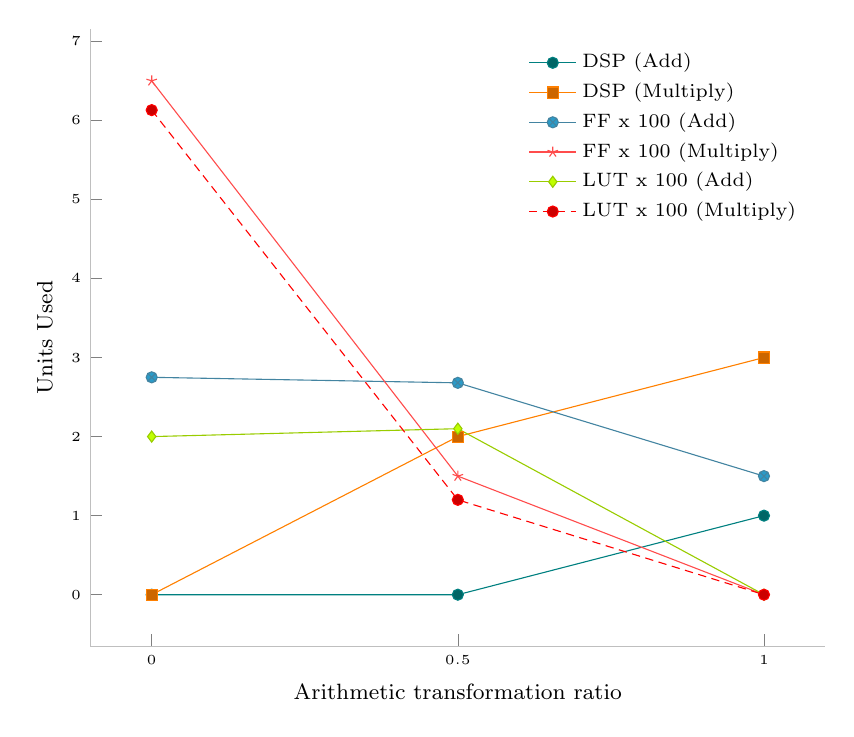
\begin{tikzpicture}
      \begin{axis}[
        cycle list name=exotic,
        xmin=0,
        ymin=0,
        axis y line*=left,
        axis x line* =bottom,
        xlabel=Arithmetic transformation ratio,
        ylabel=Units Used,
        xtick={0, 0.5, 1},
        legend columns=1,
        legend entries={
          DSP (Add),
          DSP (Multiply),
          FF x 100 (Add),
          FF x 100 (Multiply),
          LUT x 100 (Add),
          LUT x 100 (Multiply),
        },
        legend style={
          draw=none,
          cells={anchor=west}
        }
        ]
        \addplot coordinates {
          (0, 0)
          (0.5, 0)
          (1, 1)
        };
        \addplot coordinates {
          (0, 0)
          (0.5, 2)
          (1, 3)
        };
        \addplot coordinates {
          (0, 2.75)
          (0.5, 2.68)
          (1, 1.50)
        };
        \addplot coordinates {
          (0, 6.5)
          (0.5, 1.5)
          (1, 0)
        };
        \addplot coordinates {
          (0, 2)
          (0.5, 2.1)
          (1, 0)
        };
        \addplot coordinates {
          (0, 6.13)
          (0.5, 1.2)
          (1, 0)
        };
      \end{axis}
    \end{tikzpicture}
  \end{figure}
\end{frame}

\begin{frame}{4. Evaluation}
  \framesubtitle{4.4 RTM Word Length Exploration}
  \begin{figure}
    \centering
    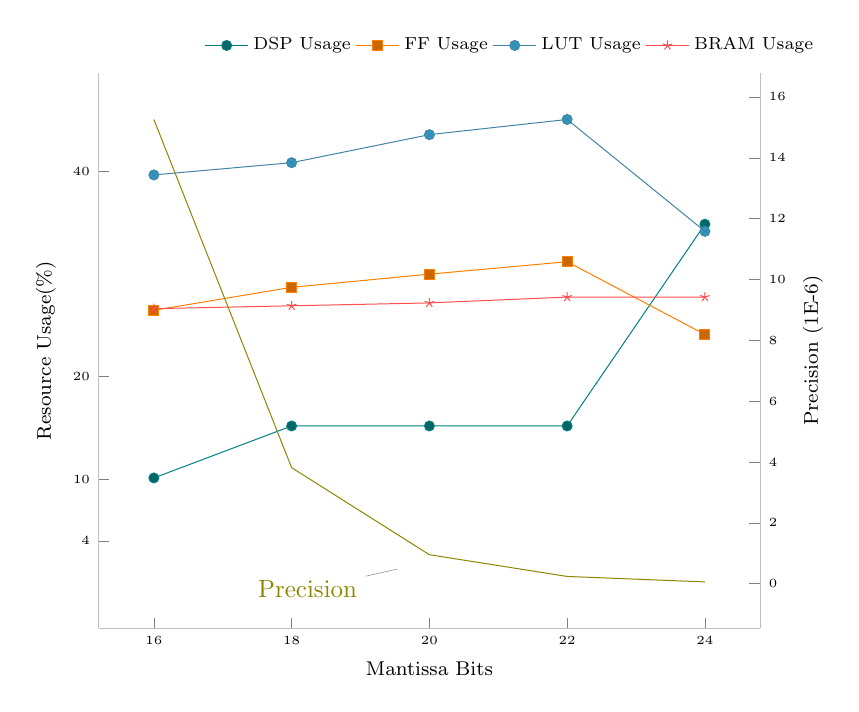
\begin{tikzpicture}[scale=0.9]
      \begin{axis}[
        cycle list name=exotic,
        ymin=0,
        axis y line*=left,
        axis x line*=bottom,
        xlabel=Mantissa Bits,
        ylabel=Resource Usage(\%),
        xtick=data,
        ytick={4, 10, 20, 40, 50, 70, 80, 100},
        legend columns=4,
        legend entries={
          DSP Usage,
          FF Usage,
          LUT Usage,
          BRAM Usage},
        legend style={
          draw=none,
          anchor=east,
          at={(1.1, 1.05)}
        }
        ]
        \addplot coordinates {
          (24, 34.82)
          (22, 15.18)
          (20, 15.18)
          (18, 15.18)
          (16, 10.12)
        };
        \addplot coordinates {
          (24, 24.09)
          (22, 31.17)
          (20, 29.96)
          (18, 28.68)
          (16, 26.44)
        };
        \addplot coordinates {
          (24, 34.13)
          (22, 45.02)
          (20, 43.54)
          (18, 40.81)
          (16, 39.62)
        };
        \addplot coordinates {
          (24, 27.73)
          (22, 27.73)
          (20, 27.16)
          (18, 26.88)
          (16, 26.60)
        };
      \end{axis}
      \begin{axis}[
        ylabel=Precision (1E-6),
        axis y line*=right,
        axis x line=none,
        ]
        \addplot[color=olive] coordinates {
          (16, 15.2585)
          (18, 3.8146)
          (20, 0.9536)
          (22, 0.2394)
          (24, 0.0596)
        } node [pos=0.8,pin={190:Precision},inner sep=20pt] {};
      \end{axis}
    \end{tikzpicture}
  \end{figure}
\end{frame}

\begin{frame}{4. Evaluation}
  \framesubtitle{4.5  RTM Parallelism}
  \begin{figure}
    \centering
    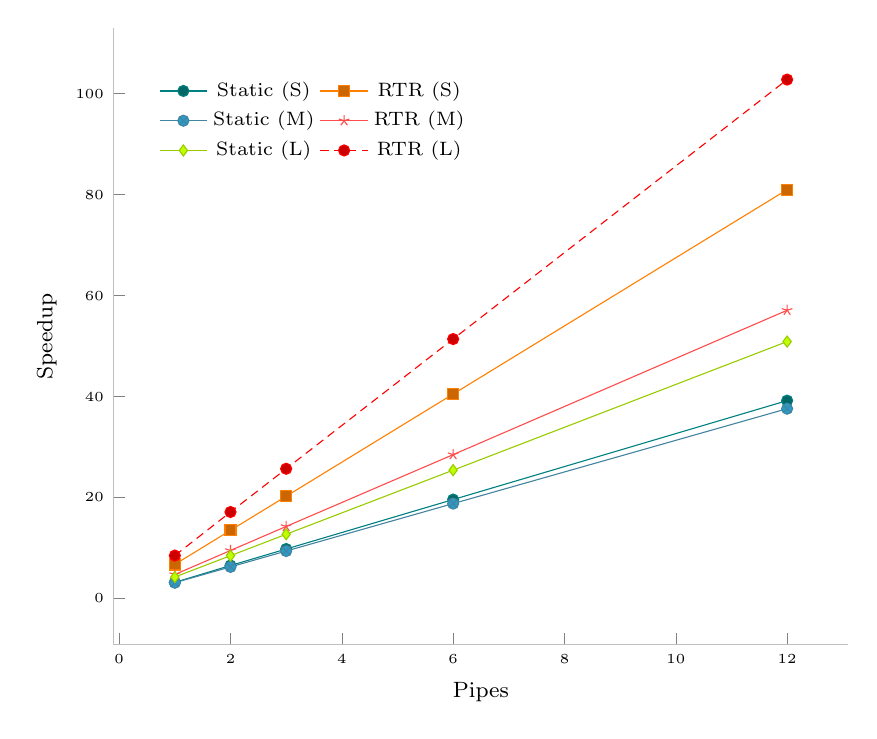
\begin{tikzpicture}
      \begin{axis}[
        cycle list name=exotic,
        xmin=1,
        ymin=1,
        xlabel=Pipes,
        ylabel=Speedup,
        axis x line* =bottom,
        axis y line* = left,
        legend columns=2,
        legend entries={
          Static (S),
          RTR (S),
          Static (M),
          RTR (M),
          Static (L),
          RTR (L)},
        legend style={
          draw=none,
          at={(0.05,0.85) },
          anchor=west
        }
        ]
        \addplot coordinates {
          (1, 3.2)
          (2, 6.53)
          (3, 9.8)
          (6, 19.6)
          (12, 39.2)
        };
        \addplot coordinates {
          (1, 6.75)
          (2, 13.5)
          (3, 20.25)
          (6, 40.5)
          (12, 81)
        };
        \addplot coordinates {
          (1, 3.13)
          (2, 6.26)
          (3, 9.4)
          (6, 18.8)
          (12, 37.6)
        };
        \addplot coordinates {
          (1, 4.75)
          (2, 9.51)
          (3, 14.27)
          (6, 28.5)
          (12, 57.1)
        };
        \addplot coordinates {
          (1, 4.25)
          (2, 8.48)
          (3, 12.725)
          (6, 25.42)
          (12, 50.9)
        };
        \addplot coordinates {
          (1, 8.5)
          (2, 17.13)
          (3, 25.7)
          (6, 51.4)
          (12, 102.8)
        };
      \end{axis}
    \end{tikzpicture}
  \end{figure}

\end{frame}

\begin{frame}{4. Evaluation}
  \framesubtitle{4.6 Performance}

  {\small
    \begin{table}
      \renewcommand{\arraystretch}{1.4}
      \begin{tabular}{c|c|c|p{1cm}|p{1cm}|p{1cm}|p{1cm}}
                   & \textbf{CPU} & \textbf{GPU} & \textbf{FPGA S (M)} & \textbf{FPGA S (A)} & \textbf{FPGA D (M)} & \textbf{FPGA D (A)} \\
        \hline \hline
        Freq.(GHz) & 2.7          & 1.15         & 0.1                 & 0.1                 & 0.1                 & 0.1                 \\
        Time (s)   & 1458         & 52           & 18                  & 18.3                & 13.4                & 13.6                \\
        GFLOP/s    & 0.9          & 51.2         & 68.0                & 66.8                & 91.6                & 90.2              \\
        Speed-up   & 1x           & 56.8X        & 76.4X               & \textbf{74.22X}              & 102.9X              & \textbf{101.3X}              \\
        Power (W)  & 185          & n / a        & 129                 & 126                 & 128                 & 125                 \\
        Efficiency & 4.9          & n / a        & 527.1               & 527.7               & 715.6               & 721.6               \\
        Eff. Gains & 1X           & n / a        & 107.5X              & \textbf{107.0X}              & 146.0X              & \textbf{147.1X}              \\
      \end{tabular}
    \end{table}
  }

  \begin{itemize}
  \item > 97\% performance of manual FPGA design
  \item > 99\% energy efficiency of manual FPGA design
  \item functionally identical dataflow design
  \end{itemize}
\end{frame}

\begin{frame}{4. Evaluation}
  \framesubtitle{4.7 RTM Discussion}
  Evaluation results show that aspect descriptions can effectively:
  \begin{itemize}
    \setlength{\itemsep}{10pt}
  \item \textbf{control DSP mapping} -- improved timing, reduced build time vs
    increased parallelism (when DSP bound)
  \item \textbf{control word length} -- increased accuracy vs reduced
    resource usage
  \item \textbf{reveal unintuitive results} -- 2 times more
    parallelism with small impact on accuracy by reducing mantissa
    from 24 bits to 22 bits
  \item \textbf{control design parallelism} -- explore increased
    performance vs increased compilation time
  \end{itemize}
\end{frame}

\begin{comment}
  \begin{frame}{4. Evaluation: Reverse Time Migration}
    \begin{table}
    \end{table}
  \end{frame}
\end{comment}

\begin{frame}{4. Evaluation}
  \framesubtitle{4.8 Application Benchmark Results}
  Comparing manual MaxCompiler designs to FAST designs:
  {\footnotesize
    \begin{table}
      \renewcommand{\arraystretch}{1.5}
      \begin{tabular}{l|c|c|c|c}
        \textbf{Kernel} & \textbf{LOC\footnote{LOC = Lines of Code}} & \textbf{API Calls} & \textbf{Performance}              & \textbf{Resource}
        \\
        \hline\hline
        CmdRead         & 1.76               & 4.33                     & \multirow{2}{1.5cm}{$ > 75\%$}        & \multirow{6}{1.5cm}{$\approx 100\%$} \\
        CmdWrite        & 1.45               & 4.13                     &                                   &                              \\
        \cline{1-4}
        RTM             & 1.17               & 10                       & \multirow{5}{1.5cm}{$ \approx 100\%$} &                              \\
        SGSmooth        & 1.85               & 14                       &                                   &                              \\
        SGDifff         & 1.75               & 14                       &                                   &                              \\
        Black-Scholes   & 2.51               & 5.5                      &                                   &                              \\
        \cline{5-5}
        Add Prediction  & 1.67               & 16                       &                                   &    $ \approx 123 \% $                          \\
      \end{tabular}
    \end{table}}

\end{frame}
\section{Conclusions}



\begin{frame}{Summary}
  \begin{beamerboxesrounded}{Contributions}
    \begin{itemize}
    \item  Aspect-driven approach and classes of aspect descriptions
    \item  FAST language and compiler
    \end{itemize}
  \end{beamerboxesrounded}
  \vspace{0.3cm}
  \begin{beamerboxesrounded}{Results}
    \begin{itemize}
    \item fastest and most energy efficient RTM design
    \item up to 60\% code reduction, 4 -- 16 times less API calls
    \item techniques deployed in FP7 HARNESS
    \item best paper candidate at ASAP'13
    \end{itemize}
  \end{beamerboxesrounded}
  \vspace{0.3cm}

  \begin{beamerboxesrounded}{Further Work}
    \begin{itemize}
    \item Intelligent design space exploration
    \item Automated partitioning of applications
    \item Automated compilation of high-level descriptions
    \item Cover heterogeneous systems (FPGAs, GPUs, CPUs)
    \end{itemize}
  \end{beamerboxesrounded}
\end{frame}



\begin{frame}{References}
  {\footnotesize
  \begin{thebibliography}{1}
  \bibitem{himeno} Phillips, Everett H., and Massimiliano
    Fatica. \emph{Implementing the Himeno benchmark with CUDA on GPU
    clusters.} Parallel \& Distributed Processing (IPDPS), 2010 IEEE
    International Symposium on. IEEE, 2010.
  \bibitem{datta} Datta, Kaushik, et al. \emph{Stencil computation
      optimization and auto-tuning on state-of-the-art multicore
      architectures.} Proceedings of the 2008 ACM/IEEE conference on
    Supercomputing. IEEE Press, 2008.
  \bibitem{cirque}Yang, Yang, et al. \emph{A hybrid circular queue method
    for iterative stencil computations on GPUs.} Journal of Computer
    Science and Technology 27.1 (2012): 57-74.
  \bibitem{arraya} Araya-Polo, Mauricio, et al. \emph{Assessing
      accelerator-based HPC reverse time migration.} Parallel and
    Distributed Systems, IEEE Transactions on 22.1 (2011): 147-162.
  \bibitem{xinyu} Niu, Xinyu, et al. \emph{Exploiting run-time
    reconfiguration in stencil computation.} Field Programmable Logic
    and Applications (FPL), 2012 22nd International Conference
    on. IEEE, 2012.
  \end{thebibliography}
  }

\end{frame}

\end{document}
